\section*{LUYỆN TẬP CHUNG}
%%==========Bài 1
\begin{bt} 
	\immini{Cho tam giác nhọn $ABC$ cân tại $A$. Từ $B$ và $C$ kẻ lần lượt hai đường cao $BH$ và $CK$ của tam giác $ABC$.
	\begin{enumerate}
	\item Chứng minh rằng đường tròn tâm $O$ đường kính $BC$ đi qua $K$ và $H$.
	\item Chứng minh rằng hai cung nhỏ $BH$ và $CK$ bằng nhau.
	\item Tính số đo của cung nhỏ $KH$ nếu $\widehat{BAC}=40^{\circ}$.
	\end{enumerate}}{\begin{tikzpicture}[line join = round, line cap = round,>=stealth,font=\footnotesize,scale=0.7]
	\def\a{4} %cạnh đáy
	\def\g{65}
	\path (0,0) coordinate (B)
	(0:\a) coordinate (C)
	($(B)!0.5!(C)$) coordinate (I) % Lấy trung điểm 
	(0:\a/2) ++(90:1) coordinate (a1)
	(\g:1) coordinate (a2)
	(intersection of B--a2 and I--a1) coordinate (A) % Giao điểm của hai đường thẳng
	($(B)!0.5!(C)$) coordinate (O)	% Lấy trung điểm
	($(A)!(C)!(B)$) coordinate (K)	% ($(B)!(A)!(C)$) Hình chiếu của A lên BC
	($(A)!(B)!(C)$) coordinate (H)	% ($(B)!(A)!(C)$) Hình chiếu của A lên BC	
	;
	\draw[thick] (A)--(B)--(C)--cycle (B)--(H)--(O) (C)--(K)--(O);
	\draw pic[angle radius=2mm,draw=black,angle eccentricity=1.5] {right angle = B--K--C};
	\draw pic[angle radius=2mm,draw=black,angle eccentricity=1.5] {right angle = B--H--C};
	\draw[thick] (B) arc (-180:180:2);
	\foreach \i/\g in {A/90,B/-135,C/-45,K/135,H/45,O/-90}{\draw[fill=black](\i) circle (1.3pt) ($(\i)+(\g:2mm)$) node[scale=1]{$\i$};}
\end{tikzpicture}}
	\loigiai{
	\begin{enumerate}
	\item Đặt $R=\dfrac{BC}{2}=OB=OC$. \\
	Khi đó $(O; R)$ là đường tròn đường kính $BC$. Dễ thấy $HO$ là trung tuyến ứng với cạnh huyền của tam giác vuông $HBC$ nên $OH=\dfrac{BC}{2}=R$. \\
	Do đó $H\in(O; R)$. \\
	Tương tự, ta cũng có $K\in(O; R)$. \\
	Vậy đường tròn $(O; R)$ đi qua các điểm $K$ và $H$.
	\item Hai tam giác vuông $H B C$ và $K C B$ có chung cạnh huyền $B C$ và $\widehat{A B C}=\widehat{A C B}$ (do tam giác $A B C$ cân tại $A$) nên $\triangle H B C=\triangle K C B$, suy ra $B H=C K$. \\
	Do đó $\triangle B O H=\triangle C O K$ (vì $B O=C O, O H=O K, B H=C K)$. \\
	Từ đó ta có $\widehat{B O H}=\widehat{C O K}$. \\
	Mặt khác, $\text{sđ }\wideparen{B H}=\widehat{B O H}$, $\text{sđ }\wideparen{C K}=\widehat{C O K}$, do đó $\text{sđ }\wideparen{B H}=\text{sđ }\wideparen{C K}$. 
	\item Ba tam giác cân $A B C$, $O C H$ và $O B K$ có các góc ở đáy bằng nhau nên ba góc ở đỉnh cūng bằng nhau. Bởi vậy ta có 
	$$
	\widehat{B O K}=\widehat{H O C}=\widehat{B A C}=40^{\circ} .
	$$
	Mặt khác, $\widehat{B O K}+\widehat{K O H}+\widehat{H O C}=\widehat{B O C}=180^{\circ}$. Do đó
	$$
	\widehat{K O H}=180^{\circ}-\widehat{B O K}-\widehat{H O C}=100^{\circ} .
	$$
	Do $\widehat{K O H}$ là góc ở tâm khác góc bẹt nên $\text{sđ }\wideparen{K H}$ là cung nhỏ. \\
	Do đó $\text{sđ }\wideparen{K H}=\widehat{K O H}=100^{\circ}$.
	\end{enumerate}
	}
\end{bt}
%%==========Bài 2
\begin{bt}
	\immini{Ta gọi hình giới hạn bởi một cung nhỏ của một đường tròn và dây căng cung đó là hình viên phân. Lập công thức tính diện tích hình viên phân ứng với cung $90^{\circ}$, biết bán kính của đường tròn là $R$.}{\begin{tikzpicture}[line join = round, line cap = round,>=stealth,font=\footnotesize,scale=1]
	\def\R{1.5}
	\path 
	(0:0) coordinate (O)
	+(45:\R) coordinate (A)
	+(-45:\R) coordinate (B);
	\draw (O) circle (\R);
	\fill[pattern = north east lines] (O)--(B) arc (-45:45:\R)--(B)--cycle;
	\draw[fill=white] (A)--(B)--(O)--cycle node[midway,sloped, shift=(90:2mm)]{$R$}
	pic[draw,thin,angle radius=2mm] {right angle = B--O--A} % Đánh dấu góc vuông	
	;
	%\draw pic[draw, angle radius = 10pt, "$60^\circ$", angle eccentricity = 2]{ angle = A--O--B};
	\foreach \x/\g in {O/180,A/45,B/-45}
	\fill (\x) circle (1.3pt)
	+(\g:2mm) node {$\x$};
	\end{tikzpicture}}
	\loigiai{
	Giả sử $A B$ là cung có số đo $90^{\circ}$; $S$ là diện tích hình viên phân (phần tô đậm trên hình) và $S_q$ là diện tích của hình quạt ứng với cung đó; $S_t$ là diện tích hình tam giác $O A B$.\\
	Ta có $S_{\mathrm{q}}=\dfrac{90}{360} \pi R^2=\dfrac{1}{4} \pi R^2, S_{\mathrm{t}} =\dfrac{1}{2} O A \cdot O B=\dfrac{1}{2} R^2$. Do đó\\
	$S =S_{\mathrm{q}}-S_{\mathrm{t}}=\dfrac{1}{4} \pi R^2-\dfrac{1}{2} R^2=R^2\left(\dfrac{\pi}{4}-\dfrac{1}{2}\right)$.
	}
\end{bt}
%%==========Bài 3
\begin{bt}%Dang toán điển hình VD7/274
	Cho $\triangle ABC$ vuông tại $A$ có $AB=10$ m, $B=60^\circ$. Vẽ nửa đường tròn $(O)$ đường kính $BC$ và đi qua điểm $A$. Tính tổng diện tích hai hình viên phân ứng với cung $AB$ và $AC$.
	\loigiai{
	\immini{Tổng diện tích hai hình viên phân bằng diện tích nửa hình tròn trừ đi diện tích $\triangle ABC$.\\
	Diện tích nửa hình tròn: $\dfrac{\pi \cdot OB^2}{2}=\dfrac{\pi \cdot 100}{2}=50\pi$ (m$^2$).\\
	Với $\triangle ABC$ ta có $AC=AB\cdot \tan 60^\circ =10\sqrt{3}$ m; $BC=2AB=20$ m.
	$$S_{\triangle ABC}=\dfrac{1}{2}AB\cdot AC=\dfrac{1}{2}\cdot10\cdot 10\sqrt{3} =50\sqrt{3}\,\,(\text{m}^2).$$
	Tổng diện tích hai hình viên phân là
	$50\pi -50\sqrt{3}=50(\pi-\sqrt{3})\,\,(\text{m}^2).$}{\begin{tikzpicture}[scale=1,font=\footnotesize,line join=round, line cap=round,>=stealth]
	\tkzDefPoints{0/0/O, 2/0/B}
	\tkzCalcLength[cm](O,B)
	\tkzGetLength{r}
	%\tkzDrawCircle[R](A,\r cm)
	\tkzDefPointBy[rotation = center O angle 60](B)
	\tkzGetPoint{A}
	\tkzDefPointBy[rotation = center O angle 180](B)
	\tkzGetPoint{C}
	\path[draw,pattern=north east lines,pattern color=gray!50!brown] (B) arc(0:60:\r)--(B);
	\path[draw,pattern=north east lines,pattern color=gray!50!brown] (A) arc(60:180:\r)--(A);
	\draw (B) arc(0:180:\r)--(B);
	\draw (O) node[below]{$O$};
	\draw (C) node[below]{$C$};
	\draw (B) node[below]{$B$};
	\draw (A) node[above]{$A$};
	\draw (O)--(A);
	\tkzDrawPoints[fill=black](O,A,B,C)
	\end{tikzpicture}}
	}
\end{bt}
%%==========Bài 4
\begin{bt}
	Cho dây $AB$ không qua tâm của đường tròn $(O)$. Gọi $A'$ và $B'$ là hai điểm lần lượt đối xứng với $A$ và $B$ qua $O$. Hỏi đường trung trực của $A' B'$ có phải là trục đối xứng của $(O)$ hay không? Tại sao?
	\loigiai{
	\immini{
	$A'$ và $B'$ là hai điểm lần lượt đối xứng với $A$ và $B$ qua $O$ suy ra $A'$ và $B'$ đều thuộc $(O)$.\\
	Gọi $d$ là đường trung trực của $A'B'$, mà $\triangle OA'B'$ cân tại $O$ ($OA'=OB'=R$).\\
	Suy ra $d$ đi qua $O$ hay $d$ chứa đường kính của $(O)$.\\
	Vậy $d$ là một trục đối xứng của $(O)$.}{
	\begin{tikzpicture}[scale=0.8]
	\def\r{2}
	\path
	(0,0) coordinate (O)
	(0:\r) coordinate (A)
	(70:\r) coordinate (B)
	($(A)!2!(O)$) coordinate (A')
	($(B)!2!(O)$) coordinate (B')
	($(A')!(O)!(B')$) coordinate (I)
	;
	\draw (O) circle (\r);
	\draw (A)--(B)--(O)--(B')--(A')--cycle;
	\draw (A)--(O)--(A') ($(O)!1.5!(I)$)--($(I)!2.6!(O)$)node[above]{$d$}
	pic[draw,thin,angle radius=2mm] {right angle = B'--I--O} % Đánh dấu góc vuông
	;
	\foreach \p/\r in {O/-70,A/0,B/60,B'/-100,A'/190,I/90}
	\fill (\p) circle (1.3pt) node[shift={(\r:2mm)}]{$\p$};
	\end{tikzpicture}
	}
	}
\end{bt}
%%==========Bài 5
\begin{bt}
	Cho tam giác $ABC$ không là tam giác vuông. Gọi $H$ và $K$ là chân các đường vuông góc lần lượt hạ từ $B$ và $C$ xuống $AC$ và $AB$. Chứng minh rằng:
	\begin{enumerate}
	\item Đường tròn đường kính $BC$ đi qua các điểm $H$ và $K$;
	\item $KH< BC$.
	\end{enumerate}
	\loigiai{
	\begin{enumerate}
	\item Đặt $R=\dfrac{BC}{2}=OB=OC$. 
	\immini{
	Khi đó $(O; R)$ là đường tròn đường kính $BC$. \\
	Xét $\triangle BHC$ có $HO$ là trung tuyến ($O$là trung điểm $BC$) suy ra \\ 
	$HO = OB = \dfrac{1}{2} BC=R$.\\ 
	Do đó $H\in(O; R)$. \\
	Xét $\triangle BKC$ vuông tại $K$ có $KO$ là trung tuyến ($O$ là trung điểm $BC$) suy ra \\ 
	$KO = OB = \dfrac{1}{2} BC=R$.\\ 
	Do đó $K\in(O; R)$. \\
	Vậy đường tròn $(O; R)$ đi qua các điểm $K$ và $H$.
	\item Xét $(O)$ có $BC$ là đường kính, $KH$ là dây không qua tâm suy ra $KH<BC$.
	}{
	\begin{tikzpicture}[line join = round, line cap = round,>=stealth,font=\footnotesize,scale=1]
	\path (0,0) coordinate (B)
	(0:4) coordinate (C) 
	(65:3) coordinate (A)
	($(A)!(C)!(B)$) coordinate (K)	% ($(B)!(A)!(C)$) Hình chiếu của A lên BC
	($(A)!(B)!(C)$) coordinate (H)	% ($(B)!(A)!(C)$) Hình chiếu của A lên BC	
	($(B)!0.5!(C)$) coordinate (O)	% Lấy trung điểm
	;
	\draw[thick] (A)--(B)--(C)--cycle (B)--(H)--(O) (C)--(K)--(O);
	\draw pic[angle radius=2mm,draw=black,angle eccentricity=1.5] {right angle = B--K--C};
	\draw pic[angle radius=2mm,draw=black,angle eccentricity=1.5] {right angle = B--H--C};
	\draw[thick] (B) arc (-180:180:2);
	\foreach \i/\g in {A/90,B/-135,C/-45,K/135,H/45,O/-90}{\draw[fill=black](\i) circle (1.3pt) ($(\i)+(\g:2mm)$) node[scale=1]{$\i$};}
	\end{tikzpicture}
	}
	\end{enumerate}
	}
\end{bt}
%%==========Bài 6
\begin{bt}
	Có thể xem guồng nước (còn gọi là cọn nước) là một công cụ hay cổ máy có dạng hình tròn, quay được nhờ sức nước chảy. Guồng nước thường thấy ở các vùng miền núi. Nhiều guồng nước được làm bằng tre, dùng để đưa nước lên ruộng cao, giã gạo hoặc làm một số việc khác.\\
	Giả sử ngấn nước ngăn cách giữa phần trên và phần dưới nước của một guồng nước được biểu thị bởi cung ứng với một dây dài $4 $ m và điểm ngập sâu nhất là $0{,}5 $ m (trên hình điểm ngập sâu nhất là điểm $C$ ta có $AB=4 $ m và $HC=0{,}5 $ m). Dựa vào đó, em hãy tính bán kính của guồng nước.
	\begin{center}
	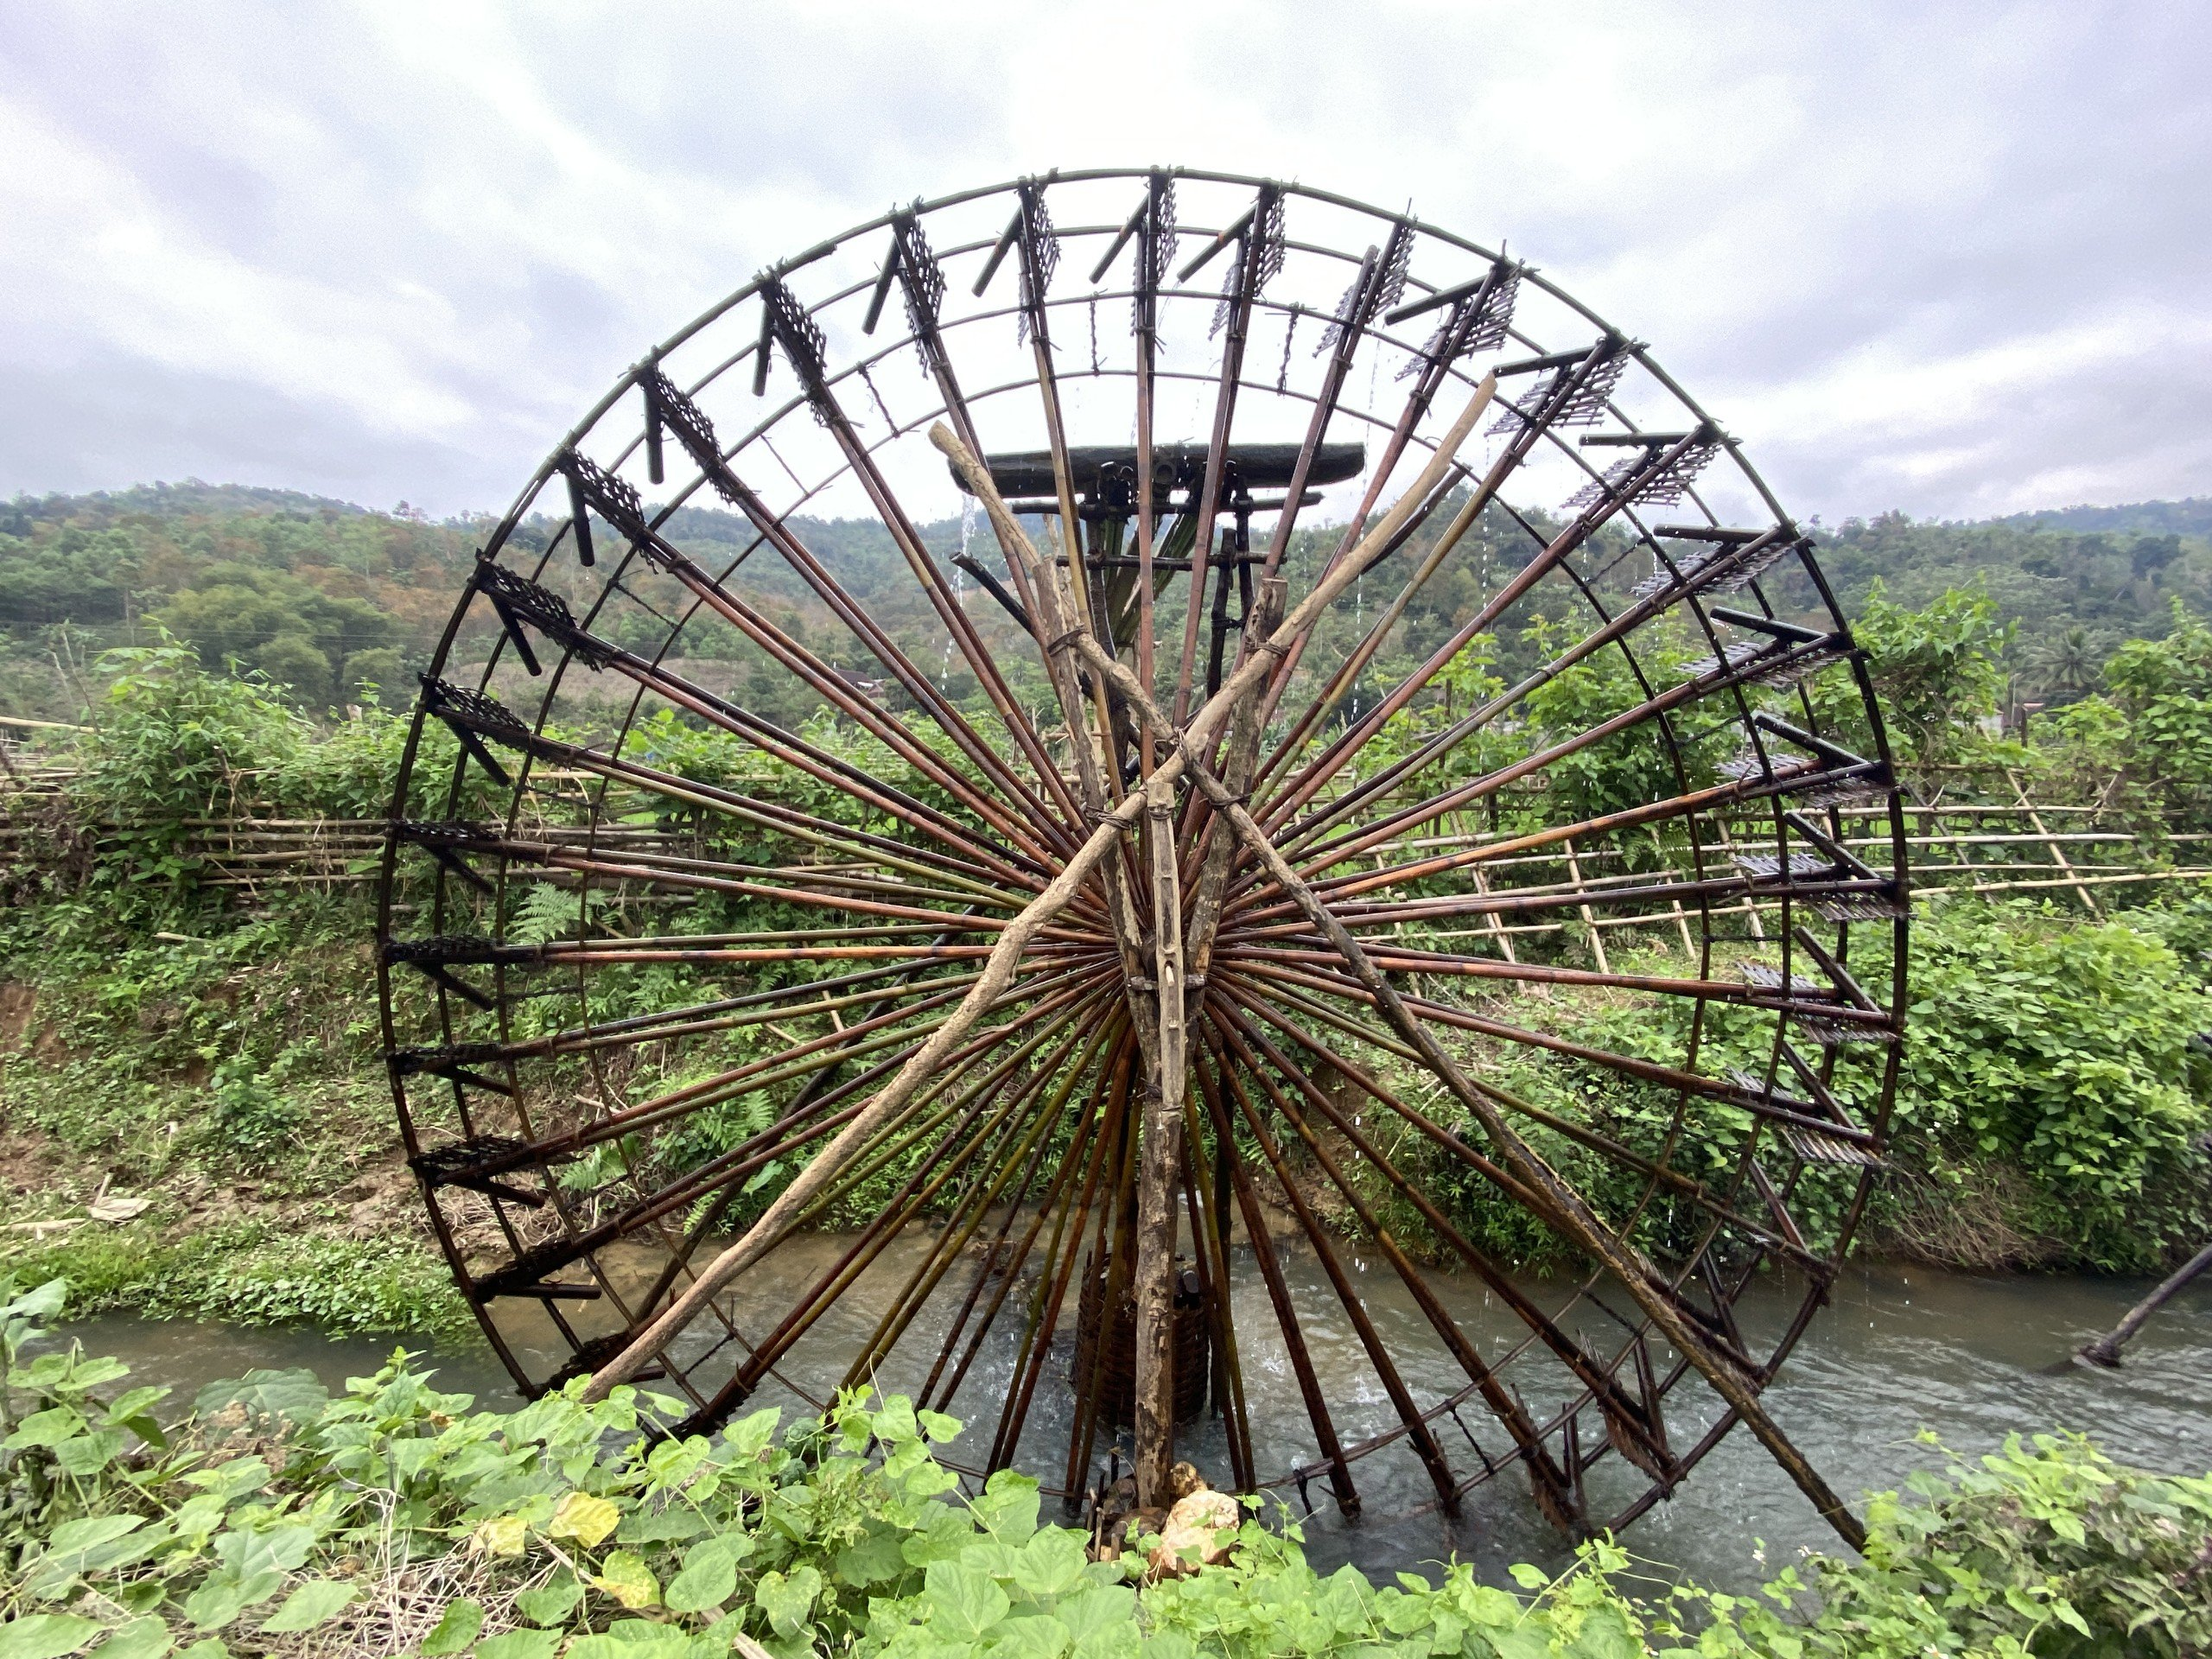
\includegraphics[scale=0.07]{images/9T5-15-LT-1.jpg}\hspace*{1cm}
	\begin{tikzpicture}[line join = round, line cap = round,>=stealth,font=\footnotesize,scale=1]
	\def\R{2}
	\path
	(0,0) coordinate (O)	% Gán tọa độ cho điểm O
	(-120:\R) coordinate (A)
	(-90:\R) coordinate (C)
	(-60:\R) coordinate (B)
	(intersection of O--C and A--B) coordinate (H)	% Giao điểm của hai đường thẳng
	;
	\draw (0,0) circle (\R)
	(A)--(O)--(C) (B)--(O)
	($(A)!1.3!(B)$)--($(B)!1.3!(A)$)
	pic[draw,thin,angle radius=2mm] {right angle = O--H--A} % Đánh dấu góc vuông
	;
	\foreach \x/\g in {O/90,A/-110,B/-45,C/-90,H/45}
	{\draw [fill=black](\x) circle (1.3pt) +(\g:2mm)node{$\x$};}
	\end{tikzpicture}
	\end{center}
	\loigiai{
	\immini{Kẻ đường kính $CT$ của $(O)$.\\
	Xét $(O)$ có $CT$ là đường kính, $A \in (O)$.\\
	Suy ra $\triangle ACT$ vuông tại $A$, suy ra.\\
	$AC^2=AH^2+HC^2$ (định lý Py-ta-go) hay $AC^2=2^2+0{,}5^2=4{,}25$.\\
	Xét $\triangle AOB$ cân tại $O$ ($OA=OB=R$) có $OH$ là đường cao nên cũng là trung tuyến.\\
	Suy ra $H$ là trung điểm $AB \Rightarrow AH=\dfrac{1}{2}AB=4:2 =2 $ m.\\
	Xét $\triangle ACT$ vuông tại $A$ có $AH$ là đường cao ($AH \perp CT$ tại $H$) suy ra \\ 
	$AC^2 = CH \cdot CT$ (hệ thức lượng).\\
	$4{,}25=0{,}5 \cdot CT$ hay $CT=8{,}5$ m.\\
	Vậy bán kính của guồng nước là $R=CT : 2=4{,}25$ m.}
	{\begin{tikzpicture}[line join = round, line cap = round,>=stealth,font=\footnotesize,scale=1]
	\def\R{2.2}
	\path
	(0,0) coordinate (O)	% Gán tọa độ cho điểm O
	(-120:\R) coordinate (A)
	(-90:\R) coordinate (C)
	(-60:\R) coordinate (B)
	(intersection of O--C and A--B) coordinate (H)	% Giao điểm của hai đường thẳng
	($(C)!2!(O)$) coordinate (T)	% ($(A)!2!(B)$) A, B đối xứng qua O
	;
	\draw (0,0) circle (\R)
	(A)--(O)--(C) (B)--(O) (C)--(A)--(T)--(O)
	($(A)!1.3!(B)$)--($(B)!1.3!(A)$)
	pic[draw,thin,angle radius=2mm] {right angle = O--H--A} % Đánh dấu góc vuông
	pic[draw,thin,angle radius=2mm] {right angle = C--A--T} % Đánh dấu góc vuông
	;
	\foreach \x/\g in {O/45,A/-110,B/-45,C/-90,H/45,T/90}
	{\draw [fill=black](\x) circle (1.3pt) +(\g:2mm)node{$\x$};}
	\end{tikzpicture}}	
	}
\end{bt}
%%==========Bài 7
\begin{bt}
	Ba bộ phận truyền chuyển động của một chiếc xe đạp gồm một giò đĩa (bánh răng gắn với bàn đạp), một chiếc líp (cũng có dạng bánh răng) gắn với bánh xe và bộ xích. Biết rằng giò đĩa có bán kính $15 $ cm, líp có bán kính $4 $ cm và bánh xe có đường kính $65 $ cm. Hỏi khi người đi xe đạp một vòng thì xe chạy được quãng đường dài bao nhiêu mét (làm tròn đến hàng phần chục)?
	\begin{center}
	\begin{tikzpicture}
	\tikzset{xedap/.pic={
	\shade[shading=radial] (-1.5,-2) rectangle (1.5,-1.6);
	\shade[shading=radial] (4.5,-2) rectangle (7.5,-1.6);
	\def\Radius{1.5cm}
	\foreach \a in {0, 10, ..., 350} {
	\draw[red] (0, 0) -- (\a:\Radius);
	\draw[black] (0, 0) -- (\a+1.5:\Radius);
	\draw[gray] (0, 0) -- (\a+3:\Radius);
	\draw[gray!50] (0, 0) -- (\a+4.5:\Radius);
	\draw[blue] (0, 0) circle[radius=\Radius];
	\draw[line width=4pt] (0, 0) circle[radius=\Radius+0.15cm];
	}
	\foreach \h in {0, 60, ..., 300} {
	\draw[color=black,line width=0.5mm,rotate around={\h:(0,0)}] (0,0) edge[-,bend left=40] (0.2cm,0) edge[-,bend right=40] (0.2cm,0);
	}
	\draw[line width=1pt] (0,0) circle[radius=0.2cm];
	\draw[line width=4pt,rounded corners=1pt,rotate=0] (1.68,0.6)--(1.94,0.54);
	\draw[line width=0.2mm,yellow!60!black] (1.8,0) arc (0:150:1.8cm)--(0,0);
	\draw[line width=0.5mm,yellow!60!black] (1.8,0) arc (0:160:1.8cm);
	\foreach \b in {0, 10, ..., 350} {
	\draw[color=red,rotate around={\b:(6,0)}] (6, 0) -- (7.5,0);
	\draw[black,rotate around={\b+1.5:(6,0)}] (6, 0) -- (7.5,0);
	\draw[gray,rotate around={\b+3:(6,0)}] (6, 0) -- (7.5,0);
	\draw[gray!50,rotate around={\b+4.5:(6,0)}] (6, 0) -- (7.5,0);
	\draw[blue] (6, 0) circle[radius=\Radius];
	\draw[line width=4pt] (6, 0) circle[radius=\Radius+0.15cm];
	}
	\draw[line width=0.2mm,yellow!60!black] (6,1.8) arc (90:190:1.8cm)--(6,0);
	\draw[line width=0.5mm,yellow!60!black] (6,1.8) arc (90:200:1.8cm);
	\draw[line width=1pt] (0,0.2cm)--(2.2,0.5cm) (0,-0.2cm)--(2.2,-0.5cm);
	\draw[line width=2pt] (2.2,0)--(2.6,-0.6) (2.2,0)--(1.8,0.6);
	\draw[line width=1mm,rounded corners=8pt,rotate around={25:(6,0)}] (6,0)--(6,1.3cm)--++(80:2.1cm);
	\draw[line width=1mm,rounded corners=8pt,rotate around={27:(6,0)}] (6,0)--(6,1.3cm)--++(80:2.1cm);
	\draw[line width=1mm,rounded corners=8pt,rotate around={26:(6,0)}] (6,0)--(6,1.3cm)--++(80:2.1cm)coordinate(a);
	\draw[line width=1.5mm] (a)--++(-80:0.15cm)--++(0:0.5cm)--++(180:0.05cm)coordinate(b);
	\draw[line width=1.1mm,rounded corners=4pt] (b)--++(-30:0.6cm)coordinate(c)--++(-160:0.4cm) (b)--++(150:0.6cm)coordinate(d)--++(200:0.4cm);
	\draw[line width=0.4mm,rounded corners=0pt] (c)--++(-95:0.1cm)--++(-160:0.25cm) (d)--++(-95:0.1cm)--++(200:0.25cm);
	\draw[line width=2mm,rotate around={35:(2.2,0)}] (2.2,0)--++(3.7,0)--++(75:0.4cm)--++(155:3.5)coordinate(e)--(2.2,0);
	\draw[line width=1mm] (0,0)--(2.2,0) (0,0)--(45:2.5cm) (0,0)--(46.5:2.5) (0,0)--(2:2.2);
	\draw[line width=1.2mm] (e)--++(106:0.9cm)--++(-74:0.1cm)coordinate(d);
	\foreach \c in {0, 72, ..., 288} {\draw[color=red,line width=1.8mm,rotate around={\c:(2.2,0)}] (2.2,0) edge[-,bend left=30] (2.69,0);}
	\draw[line width=2pt] (2.2,0) circle[radius=0.5cm];
	\fill (2.2,0) circle[radius=0.1cm];
	\draw[line width=4pt,rounded corners=1pt,rotate=0] (2.4,-0.58)--(2.68,-0.56);
	\draw[line width=2pt] (2.2,0)--(2.6,-0.6);
	\shade[top color=white,bottom color=black,rounded corners=2pt,rotate around={10:(d)}] (d)--++(220:2mm)--++(100:2mm)--++(180:2mm)--++(110:1.5mm)--++(160:2mm)--++(110:3.5mm)coordinate(i)--++(-15:10mm)--++(-5:5mm)--++(-20:2mm)coordinate(j)--++(-50:0.7mm)--++(180:4mm)--++(170:1mm)--++(-175:2mm)--(d);
	\shade[top color=gray!50,bottom color=black,rounded corners=2pt,rotate around={10:(d)}] (d)--++(220:2mm)--++(100:2mm)--++(180:2mm)--++(110:1.5mm)--++(160:2mm)--++(110:3.5mm)--++(-50:4.5mm)--++(-3:12mm)--++(-10:2mm)--++(180:4mm)--++(170:1mm)--++(-175:2mm)--(d);
	\filldraw[black] (0,0)circle(2pt) (6,0)circle(2pt);
	\draw[line width=0.2mm] (0,0)--++(105:2cm)--++(-2:0.7cm)coordinate(g)--+(-10:1.5cm) (g)--(0,0);
	\shade[top color=gray!10!white,bottom color=gray] (-0.8cm,1.9cm)--++(-3:1.4cm) arc (-90:90: 0.4mm)--++(174:1.4cm) arc (90:270: 0.65mm);
	\shade[top color=gray!20,bottom color=black] (-0.8cm,1.9cm)--++(-3:1.4cm) arc (-90:90: 0.4mm)--++(177:1.4cm) arc (90:270: 0.4mm);	
	}}
	\path (0,0) pic[rotate=0,scale=0.8]{xedap};
	\draw [<-,thick](1.7,-0.45)--(2,-1.2) node[below,font=\scriptsize]{Giò đĩa};
	\end{tikzpicture}
	\end{center}
	\loigiai{
	Chu vi của giò đĩa là $C=2 \cdot \pi\cdot 15=30 \pi$ cm.\\
	Chu vi của líp là $C=2 \cdot \pi\cdot 4=8 \pi$ cm.\\
	Chu vi của bánh xe là $C=\pi\cdot65=65 \pi$ cm.\\
	Tỉ số chu vi của giò đĩa và chu vi của líp là $\dfrac{30 \pi}{8 \pi}=\dfrac{15}{4}$.\\
	Tỉ số vòng quay của líp và vòng quay của giò đĩa là $\dfrac{15}{4}$.\\
	Khi líp quay được $1$ vòng thì bánh xe cũng quay được $1$ vòng tương ứng.\\
	Suy ra khi giò đĩa quay $1$ vòng thì bánh xe quay được $\dfrac{15}{4}$ vòng.\\
	Khi đó mỗi điểm trên bánh xe di chuyển được quãng đường là $l=\dfrac{15}{4} \cdot65\pi\approx 765{,}8 \text{ (cm) }=7{,}7\text{ (m)}.$\\
	Vậy người đi xe đạp giò đĩa $1$ vòng liên tục thì xe đạp di chuyển được quãng đường xấp xỉ $7{,}7$ m.
	}
\end{bt}
%%==========Bài 8
\begin{bt}
	Cho tam giác đều $ABC$ có $AB=2 \sqrt{3} $ cm. Nửa đường tròn đường kính $BC$ cắt hai cạnh $AB$ và $AC$ lần lượt tại $D$ và $E$ (khác $B$ và $C$).
	\begin{enumerate}
	\item Chứng tỏ rằng ba cung nhỏ $BD$, $DE$ và $EC$ bằng nhau. Tính số đo mỗi cung ấy.
	\item Tính diện tích của hình viên phân giới hạn bởi dây $BD$ và cung nhỏ $BD$.
	\end{enumerate}
	\loigiai{
	\begin{enumerate}
	\item Xét $(O)$ có $BC$ là đường kính (giả thiết);
	$D \in (O)$ ($(O)$ cắt $AB$ tại $D$); \\
	Suy ra $\triangle BDC$ vuông tại $D$ hay $CD \perp AB$ tại $D$.\\
	Xét $(O)$ có $BC$ là đường kính (giả thiết); 
	$E \in (O)$ ($(O)$ cắt $AC$ tại $E$);
	\\
	Suy ra $\triangle BEC$ vuông tại $E$ hay $BE \perp AC$ tại $E$.\\ 
	Xét $\triangle ABC$ đều có 
	$CD$ là đường cao ($CD \perp AB$ tại $D$);
	\\
	Suy ra $CD$ là đường phân giác hay $\widehat{ACD} = \widehat{BCD}=\dfrac{1}{2} \widehat{ACB}=30^\circ$.
	\immini{
	Do đó $\widehat{ECD}=\widehat{BCD}=30^\circ$.\\
	Chứng minh tương tự $\widehat{CBE}=30^\circ$.\\
	Xét $(O)$ có 
	\begin{itemize} 
	\item[] $\widehat{ECD}=\dfrac{1}{2}\text{sđ}\wideparen{ED}$ (góc nội tiếp chắn cung $ED$). 
	\item[] $\widehat{BCD}=\dfrac{1}{2}\text{sđ}\wideparen{BD}$ (góc nội tiếp chắn cung $BD$). 
	\item[] $\widehat{BCD}=\dfrac{1}{2}\text{sđ}\wideparen{CE}$ (góc nội tiếp chắn cung $CE$). 
	\end{itemize} 
	Mà $\widehat{BCD}=\widehat{ECD}=\widehat{CBE}=30^\circ $.\\
	Vậy $\text{sđ}\wideparen{ED}=\text{sđ}\wideparen{BD}=\text{sđ}\wideparen{CE}=2 \cdot 30^\circ=60^\circ$ hay $\wideparen{ED}=\wideparen{BD}=\wideparen{CE}$.}{
	\begin{tikzpicture}[line join = round, line cap = round,>=stealth,font=\footnotesize,scale=1]
	\def\a{4} % cạnh đáy
	\def\g{60}
	\path (0,0) coordinate (B)
	(0:\a) coordinate (C);
	\coordinate (A) at ($(B)!1!60:(C)$);
	\path ($(B)!0.5!(C)$) coordinate (O) % Lấy trung điểm 
	($(A)!(C)!(B)$) coordinate (D)
	($(A)!(B)!(C)$) coordinate (E)
	;
	\draw[thick] (A)--(B)--(C)--cycle (B)--(E)--(O) (C)--(D)--(O);
	\draw pic[angle radius=2mm,draw=black,angle eccentricity=1.5] {right angle = B--D--C};
	\draw pic[angle radius=2mm,draw=black,angle eccentricity=1.5] {right angle = B--E--C};
	\draw[thick] (B) arc (-180:180:2);
	\foreach \i/\g in {A/90,B/-135,C/-45,D/135,E/45,O/-90}{\draw[fill=black](\i) circle (1.3pt) ($(\i)+(\g:2mm)$) node[scale=1]{$\i$};}
	\end{tikzpicture}
	}
	\item 
	Gọi $S$ là diện tích hình viên phân (phần tô màu trên hình) và $S_\mathrm{q}$ là diện tích của hình quạt ứng với cung đó; $S_\mathrm{t}$ là diện tích hình tam giác $O A B$.\\
	Ta có bán kính đường tròn $(O)$ là $R=\dfrac{BC}{2}=\dfrac{2\sqrt{3}}{2}=\sqrt{3}$ cm.\\
	Ta có $S_{\mathrm{q}}=\dfrac{60}{360} \pi (\sqrt{3})^2=\dfrac{1}{2} \pi$; $S_{\mathrm{t}} =OB^2 \cdot \dfrac{\sqrt{3}}{4}=(\sqrt{3})^2\dfrac{\sqrt{3}}{4}=\dfrac{3\sqrt{3}}{4}$. Do đó\\
	$S =S_{\mathrm{q}}-S_{\mathrm{t}}=\dfrac{1}{2} \pi-\dfrac{3\sqrt{3}}{4}$ cm$^2$.
	\end{enumerate}
	}
\end{bt}
%%==========Bài 9
\begin{bt}%PP giai toan VD5/150
	\immini{\everymath{\allowdisplaybreaks \displaystyle}
	Cho đường tròn có đường kính $AB$. Trên đoạn $AB$ lấy hai điểm $C$ và $D$ sao cho $AC=CD=DB$. Vẽ về một phía của $AB$ hai nửa đường tròn đường kính $AC$ và $AD$. Vẽ về phía bên khia $AB$ hai nửa đường tròn đường kính $CB$, $DB$. So sánh diện tích phần tô đen và diện tích mỗi phần còn lại.}{\begin{tikzpicture}[scale=0.7,font=\footnotesize,line join=round, line cap=round,>=stealth]
	\tkzDefPoints{0/0/O, -2/0/A, 2/0/B}
	\coordinate (C) at ($(A)!1/3!(B)$);
	\coordinate (D) at ($(A)!2/3!(B)$);
	\tkzCalcLength[cm](O,A)
	\tkzGetLength{r}
	\draw (O) circle (\r);
	\tkzDrawPoints[fill=black](O)
	\tkzLabelPoints[left](O)
	%\path[draw,pattern=north east lines,pattern color=gray!50!brown] (A) arc(180:0:2*\r/3)--(D) arc(-180:0:\r/3)--(B) arc(0:-180:2*\r/3)--(C) arc(0:180:\r/3)--cycle;
	\path[draw,fill=black] (A) arc(180:0:2*\r/3)--(D) arc(-180:0:\r/3)--(B) arc(0:-180:2*\r/3)--(C) arc(0:180:\r/3)--cycle;
	\draw (A) node[left]{$A$};
	\draw (B) node[above right]{$B$};
	\draw (C) node[below left]{$C$};
	\draw (D) node[above right]{$D$};
	\draw (A)--(B);
	%\tkzMarkAngle[arc=l,size=0.7cm](A,O,B)
	\end{tikzpicture}}
	\loigiai{
	Đặt $AC=CD=DB=2a$ thì $AB=6a$.\\
	Diện tích nửa hình tròn đường kính $AB$ là $S_1=\dfrac{1}{2}\pi (3a)^2=\dfrac{9\pi a^2}{2}$ (đvdt).\\
	Diện tích nửa hình tròn đường kính $AC=DB=2a$ là $S_2=\dfrac{1}{2}\pi a^2$ (đvdt).\\
	Diện tích nửa hình tròn đường kính $AD=CB=4a$ là $S_3=\dfrac{1}{2}\pi (2a)^2=2\pi a^2$ (đvdt).\\
	Diện tích hình tròn đường kính $AB$ là $S=\pi (3a)^2=9\pi a^2$ (đvdt).\\
	Nên diện tích mỗi phần còn lại của hình tròn bằng
	$$S_1 +S_2 -S_3= \dfrac{3\pi a^2}{2}+\dfrac{\pi a^2}{2}- 2\pi a^2=3\pi a^2 =\dfrac{1}{3}S.$$
	Diện tích phần tô đen bằng $S-\dfrac{2}{3}S=\dfrac{1}{3}S$.\\
	Vậy diện tích mỗi phần bằng $\dfrac{1}{3}$ diện tích hình tròn đường kính $AB$. }
\end{bt}